\section{Experiments}
\label{sec:eval}
To incorporate a more diverse range of styles, we gather two collections of datasets for our experiments. The first one is collected from literature translations with different writing styles as previously shown, and the second one is a grouped standard dataset comprised of several existing style transfer tasks.

We test our ST$^2$ framework and other state-of-the-art models on these two datasets, and verify the effectiveness of ST$^2$ on few-shot style transfer scheme. By comparing our framework with the pretrained base models, we further demonstrate that ST$^2$ is able to improve the performance
in terms of content preservation, language fluency and style transfer accuracy by incorporating relevant knowledge from other style transfer tasks.
%both in terms of language fluency and style transfer accuracy.



\subsection{Benchmark}

Since we extend the definition of style to the general writing style of a person, we do not need to be limited to the widely used Yelp/Amazon review and GYAFC datasets. To model the real situation where we have different style pairs with limited data for each style pair, we perform experiments on the newly constructed literature translations dataset~(LT) and a set of popular style transfer datasets with reduced sizes.
\begin{table*}[t]
	\footnotesize
	\centering
	\begin{tabular}{c|cccccc|cccccc}
		\hline
		\multirow{2}{*}{\textbf{Model}} & \multicolumn{6}{c|}{\textbf{LT}} & \multicolumn{6}{c}{\textbf{GSD}} \\
		\cline{2-13}
		& \textbf{BLEU-3}$^{\uparrow}$  & \textbf{PPL}$^\downarrow$ & \textbf{ACC}$^\uparrow$ &\textbf{G3}$^\uparrow$ &\textbf{H3}$^\uparrow$ & \textbf{Human}$^\uparrow$ & \textbf{BLEU-3}$^\uparrow$ & \textbf{PPL}$^\downarrow$ & \textbf{ACC}$^\uparrow$ &\textbf{G3}$^\uparrow$ &\textbf{H3}$^\uparrow$& \textbf{Human}$^\uparrow$ \\
		\hline
		Template & 8.10  & 5.4 & 0.3 & 4.7 &1.1 & 2.3 & 68.6 & 5.3 & 0.42 &9.2 &1.2 & 3.0 \\
		\hline

		DeleteRetrieve & 0.27 & 63.3 & 0.33 &1.3 &0.3 & 1.9 & 0.71  & 28.8 & 0.41 &1.8 &0.4 & 2.9 \\
		DualRL & 0.01 & 1400.7 & 0.49 &0.3 &0.1 & 1.9 & 5.80  & 171.0 & 0.41 &3.4 &0.4 & 2.4 \\

		B-GST & 0.56 & 24.4 &0.50  &1.8 &0.4 & 1.9  & 15.62  & 31.1 &0.36  &4.8 &0.6 & 1.9  \\

		\hline
		\underline{CrossAlign} & 0.0  & 1895.6 & 0.45 &0.0 &0.0 & 1.8 & 0.0  & 1049.7 & 0.36 &0.0 &0.0 & 1.8 \\
		ST$^2$-CA & 0.26 & 54.8 & 0.54 &1.3 &0.3 & 2.4 & \textbf{17.6} & 21.4 & 0.45 &\textbf{5.3} &0.8 & 3.3 
		\\
		\hline
		\underline{VAE} & 0.11  & 8.5 & 0.49 &1.2 &0.2 & 1.8 & 0.35 & 21.5 & 0.45 &1.5 &0.4 & 2.9 \\
		ST$^2$-VAE & 0.34  & 8.2 & \textbf{0.62} &1.9 &0.5 & 3.3 & 0.80 & 10.9 & \textbf{0.71} &2.4 &0.6 & 3.2 \\
		\hline
		\underline{CP-VAE} & 0.57 & 11.4 &0.41  &1.8 &0.5 & 2.4  & 2.52  & 8.3 &0.64  &3.8 &0.8 &3.1  \\
		ST$^2$-CP-VAE &\textbf{0.71}   &\textbf{8.1}  &0.49  &\textbf{2.3}  &\textbf{0.7} &\textbf{3.4}  &2.87  &\textbf{4.6}  &0.66  &5.0 &\textbf{1.6} &\textbf{3.5}  \\
		\hline
	\end{tabular}
	\caption{Results for multi-task style transfer. The larger$^\uparrow$/lower$^\downarrow$, the better. Our base models are underlined.}\label{tb:exp1}
\end{table*}
\begin{table}[th]\footnotesize
	\centering
	\begin{tabular}{cc}
		\hline
		\textbf{Dataset} & \textbf{Style} \\
		\hline
		Yelp & (health) positive/negative \\
		Amazon & (musical instrument) positive/negative \\
		GYAFC & (relations )formal/informal \\
		Wikipedia & standard/simple \\
		Bible & standard/easy \\
		Britannica & standard/simple \\
		Shakespeare & original/modern \\
		\hline
	\end{tabular}
	\caption{Grouped standard dataset.}\label{tb:data2}
\end{table}
\subsubsection*{Grouped Standard Datasets (GSD)}

In our second collection, we group popular datasets for style transfer~\citep{li2018delete,Sudhakar2020,rao-tetreault-2018-dear}. For large datasets, we use only a small portion of them in order to model our few-shot style transfer task. The datasets we use are listed in Table \ref{tb:data2}. For the standard/simple versions of Wikipedia, we use the aligned sentences by \citet{hwang2015aligning} for testing. For all datasets listed in the table, we use 10k sentences for training and 1k sentences for testing.


\subsection{Metrics}
%\KZ{Consider trimming down.}
\subsubsection*{BLEU-3}

To evaluate content preservation of transferred sentences, we report the BLEU score~\citep{papineni2002bleu} between reference sentences and generated sentences. When ground-truth sentences are available in the test set~(all tasks in LT, GYAFC and Wikipedia in GSD), we calculate the BLEU scores between generated sentences and ground-truth sentences. When they are missing, we calculate self-BLEU scores based on the original sentences\footnote{We use BLEU score, more specifically BLEU-3, because BLEU-4 is close to zero for most models in our experiment.}.

\subsubsection*{Perplexity (PPL)}

Following the metrics used by \citet{john2018disentangled}, we use a bigram Kneser-Key bigram language model to evaluate the fluency and naturalness of generated sentences~\citep{kneser1995improved}. The language models are trained in the target domain for each style pair. We use the training data before reduction to train the language model for GSD set.


\subsubsection*{Transfer Accuracy (ACC)}

To evaluate the effectiveness of style transfer, we pretrain a RoBERTa~\citep{liu2019roberta} classifier for each style pair. The transfer accuracy is calculated based on the prediction of the classifier. Our classifier achieves test accuracy of 80.0\% $\sim$ 97.0\% on LT(85.0\% on average) and 73.8\% $\sim$ 98.5\%(83.9\% on average) on GSD dataset, which serves as a reasonable evaluator for transfer effectiveness even for the fine-grained writing style.
%\KZ{Can we do some human eval for transfer accuracy? Not for all the datasets but for those that human can identify? But if those that human can easily identify has good automatic accuracy scores, then not much point. I think maybe you want to show the detailed transfer accuracies for each datasets, cos some of the numbers are not that high, like 67.8.}

\subsubsection*{Overall Performance}
Since it is hard to measure the transfer quality solely relying on one single metric, we perform both automatic and human evaluation to quantify the overall transfer effectiveness.
\begin{itemize}
	\item \textbf{Automatic Evaluation.}~As observed in previous literature~\citep{li2018delete,Sudhakar2020}, accuracy, BLEU score and perplexity may not correlate well with human evaluations. Therefor, it is important to not only consider them in isolation. To this end, we also report the geometric mean(\textbf{G3}) and harmonic mean(\textbf{H3}) of BLEU-3, $\frac{1}{\log{PPL}}$ and ACC to serve as two proxies of the overall performance.
	\item \textbf{Human Evaluation.}~We conduct an additional human evaluation, following \citet{luo2019dual}. For each model with each transfer direction, we randomly sample 25 sentences for human evaluation. Each annotator(two native English speakers in total) is asked to assess the overall transfer effectiveness of each output sentence at a 4-point scale by jointly considering content preservation, transfer strength and language fluency, given the source sentence and the target style\footnote{For LT collection, we additionally provide annotators with writer-specific statistics as auxiliary information.}.
	The final score for each model is calculated as the average score given by the annotators. The kappa inter-judge agreement is 0.769, indicating significant agreement.
\end{itemize}

\subsection{Baselines}
We compare the following existing state-of-the-art models against several base models~(\textbf{CrossAlign}~\citep{shen2017style},  \textbf{VAE}~\citep{john2018disentangled} and \textbf{CP-VAE}~\citep{Xu2019}) equipped with our ST$^2$ framework: \textbf{Template}-based model, \textbf{DeleteRetrieve}~\citep{li2018delete}, \textbf{DualRL}~\citep{luo2019dual}, \textbf{B-GST}\citep{Sudhakar2020}. Note that all above models except for \textbf{Template} are generative models, which means the transfered sentences are generated from scratch with a decoder.
\begin{table*}[t!]\footnotesize
	\centering
	\begin{tabular}{c|c}
		\hline
		\textbf{Original Sentence} (The Brothers Karamazov {\color{red}A R.M}$\rightarrow${\color{blue}R.P}) & \emph{but who can really tell ?} \\
		\hline
		Template & \emph{but who can really tel maybe rogozhinl?} \\
		CrossAlign & \emph{ow inside, beautiful, added how any how how how how how how} \\
		DeleteRetrieve & \emph{in the , the} \\
		DualRL & \emph{it , it , it , it , it , it} \\
		VAE & \emph{i was haunted by the way i was walking of those outbursts} \\
		B-GST & \emph{but who who who , he he was was simply simply} \\
		CP-VAE & \emph{but who is true , is not true man} \\
		\hline
		ST$^2$-CrossAlign (ours) & \emph{and also liked that she 's a thinking ?} \\
		ST$^2$-VAE (ours) & \emph{but how can tell it ?} \\
		ST$^2$-CP-VAE (ours) & \emph{ but he didn ’ t know ?} \\
		\hline
		\textbf{Target Sentence} & \emph{but who knows , perhaps he was simply naive .} \\
		\hline
		\hline
		\textbf{Original Sentence} (The Iliad {\color{red}I C.J}$\rightarrow${\color{blue}R.F}) & \emph{listen now to me .} \\
		\hline
		Template & \emph{listen now to me.} \\
		CrossAlign & \emph{beat imagine beat but rest the world,} \\
		DeleteRetrieve & \emph{to the unk of the gods , the unk of the gods ,} \\
		DualRL & \emph{swallowing swallowing swallowing swallowing swallowing} \\
		VAE & \emph{but the two aeantes kept on the tower went down on the shore} \\
		B-GST & \emph{me me me me me} \\
		CP-VAE & \emph{take me back to fight against sea tomorrow !} \\
		\hline
		ST$^2$-CrossAlign (ours) & \emph{listen to me} \\
		ST$^2$-VAE (ours) & \emph{listen to me now .} \\
		ST$^2$-CP-VAE (ours) & \emph{listen to me !} \\
		\hline
		\textbf{Target Sentence} & \emph{listen to me , quickly !} \\
		\hline
		\hline
		\textbf{Original Sentence} (GYAFC {\color{red}informal}$\rightarrow${\color{blue}formal}) & \emph{do n't even do that to yourself ! ! !} \\
		\hline
		Template & \emph{do n't even do that to yourself allow} \\
		CrossAlign & \emph{whatever you doing} \\
		CrossAlign (pretrained) & \emph{do n't even do that to do ! ! !} \\
		DeleteRetrieve & \emph{do n't let him if you are it !} \\
		DualRL & \emph{do n't even do that to yourself success ! !} \\
		VAE & \emph{do n't do anything without do things do n't do} \\
		VAE (pretrained) & \emph{do n't even that to do anything} \\
		B-GST & \emph{do n ' t even do that that ! ! !} \\
		CP-VAE & \emph{men do not have sex as a boyfriend ! } \\
		\hline
		ST$^2$-CrossAlign (ours) & \emph{do n't tell me you want to do that .} \\
		ST$^2$-VAE (ours) & \emph{you 're not really good to ask yourself to do that} \\
		ST$^2$-CP-VAE (ours) & \emph{do not allow yourself to be that way .} \\
		\hline
		\textbf{Target Sentence} & \emph{do not do that to yourself !} \\
		\hline
	\end{tabular}
	\caption{Sample outputs for the The Brothers Karamazov~({\color{red}Andrew R. MacAndrew}  $\rightarrow$ {\color{blue}Richard Pevear}) and The Iliad ~({\color{red}Ian C. Johnston} $\rightarrow$ {\color{blue}Robert Fagles}) from LT collection, GYAFC ({\color{red}informal} $\rightarrow$ {\color{blue}formal}) from GSD collection, from which we show how the proposed ST$^2$ framework is able to improve small data text style transfer in terms of content preservation, language fluency and style transfer strength.}\label{tb:qual}
\end{table*}
\subsection{Implementation Details}
In the experiment we primarily adopt CrossAlign, VAE and CP-VAE as our base models, more details regarding the base models can be found in the Appendix A. Optimizers are chosen based on the original implementation of each base model and we perform a simple grid search on development set to find the best meta training and fine-tuning learning rate in $[0.1, 0.01, 0.001]$. Other model-specific hyper-parameters are also tuned on the development set. For MAML in ST$^2$, we implement it using its first-order approximation since it is more stable and achieves comparable performance against its second-order version. All experiments are carried out using a single RTX 2080Ti GPU on Ubuntu 18.04. Our Pytorch implementation is publically available at \url{https://anonymous.for.blind.review}.

\subsection{Main Results}
\label{sec:st}

We compare the results with the state-of-the-art models for the style transfer task. All the baseline models are trained on the single style pair. The ST$^2$ model is trained on all the tasks for both LT and GSD sets, and then fine-tuned using a specific style pair in the sets. The trained meta-learner is fine-tuned on each of the sub-tasks, and the scores are calculated as the average among all sub-tasks for both ST$^2$ models and baselines. The results are shown in Table \ref{tb:exp1}.

We note that the BLEU and PPL scores for the template-based model appear
to be superior to those of other models. This is because it directly
modifies the original sentence by changing a couple of words (resulting in a large self-BLEU). So the modification
is actually minimum under the small data setting (see Table \ref{tb:qual}). However, its transfer accuracy suffers, which is
well expected. All other models are generative in nature, which makes the comparisons among them more convincing.

From the results, we notice that state-of-the-art models fail to achieve satisfying performances in our few-shot style transfer tasks, and many baseline models fail to generate syntactically or logically consistent sentences. Particularly, the BLEU score for one of our base model CrossAlign is zero. In contrast, CP-VAE, which constrains the posterior style latent space to be within a low-dimensional(less than 50) probability simplex, achieves the highest BLEU score among all generative baselines that are trained from scratch. However, even without the help of large-scale pretrained language model~(e.g., GPT in B-GST), models equipped with ST$^2$ are able to generate more fluent sentences both in terms of automatic evaluation and human evaluation, meanwhile achieving a higher transfer accuracy.  By inspecting evaluation results of all base models in Table \ref{tb:exp1} before and after being equipped with ST$^2$, we show that ST$^2$ is robust to the choice of base models as all evaluation metrics regarding transfer effectiveness obtain consistent improvement after applying ST$^2$ to the base models. It is worth noting that both CrossAlign and VAE are significantly inferior to the two state-of-the-art models B-GST and CP-VAE in terms of overall performance before the enhancement by our multi-task meta-learning framework. By incorporating related tasks into a unified transfer model, the learned parameters can be better adapted to one specific task with minimal amount of data. While ST$^2$-VAE fuses disentangled style embeddings of all instances from target corpus hence yielding better transfer strength and ST$^2$-CA tends to reconstruct the original sentence therefore achieving higher BLEU score on GSD, ST$^2$-CP-VAE learns to strike a balance and obtains the best overall performance. A similar phenomenon is also observed on LT.
%ST$^2$-CA achieves better performance on GSD because its binary style embedding mechanism suffices to transfer sentences between styles like sentiment polarity, while ST$^2$-VAE fuses disentangled style embeddings of all instances from target corpus hence yielding better transfer quality on LT.

For qualitative analysis, we randomly select transferred sentences
by baseline models, pretrained base models and our ST$^2$ models
on two sub-tasks from LT collection and one sub-task from GSD collection,
which are shown in Table \ref{tb:qual}.

We might be tempted to conclude that this is simply because the
ST$^2$ models learn better language models because they are trained on,
i.e., data from all styles rather than only a single pair of styles.
Therefore, further experiments are required.
\subsection{Pretrained Base Models}
\label{sec:pretrain}
\begin{table}[ht]\footnotesize
	\centering
	\begin{tabular}{c|cccc}
		\hline
		\textbf{Model} & \textbf{BLEU-3}$^\uparrow$ & \textbf{PPL}$^\downarrow$ & \textbf{ACC}$^\uparrow$ & \textbf{HU}$^\uparrow$ \\
		\hline
		CA$^*$ &\textbf{24.21}   & 12.2 & 0.32 & 1.9 \\
		VAE$^*$ &1.84   & 22.4 & 0.48 & 2.0 \\
		\hline
		ST$^2$-CA$^*$ &14.62   & 23.2 & 0.37 &2.2  \\
		ST$^2$-VAE$^*$ &0.95   & 10.9 & 0.66  &2.9  \\
		\hline
		ST$^2$-CA & 17.60  & 21.4 & 0.45 & 3.3 \\
		ST$^2$-VAE & 0.80  & \textbf{10.9} & \textbf{0.71} & 3.2 \\
		\hline
	\end{tabular}
	\caption{Results on GSD for pretrained ($^*$) base models ( CA means CrossAlign) and ST$^2$. HU means human evaluation on fluency/content preservation.}\label{tb:exp2}
\end{table}
Based on the previous reasoning, we extract and pretrain the language model module in two of our base models (CrossAlign and VAE) on the union of training data from all sub-tasks. Starting with a well-trained language model, we then fine-tune the models for each style transfer task. By comparing pretrained base models with our ST$^2$ models, we verify that meta-learning framework can improve the style transfer accuracy in addition to language fluency. We perform this experiment only on the GSD dataset since they are enough for analysis purposes.

In addition, to examine the effect of pretraining combined with meta-learning, we also add a pretraining phase to our ST$^2$ model. The quantitative and qualitative results are included in Table \ref{tb:exp2} and Table \ref{tb:qual} (on GSD dataset for the pretrained base models).
\begin{figure}[t!]
	\underline{\small Pretrained CrossAlign}\\
	\begin{minipage}{0.45\linewidth}
		\centering
		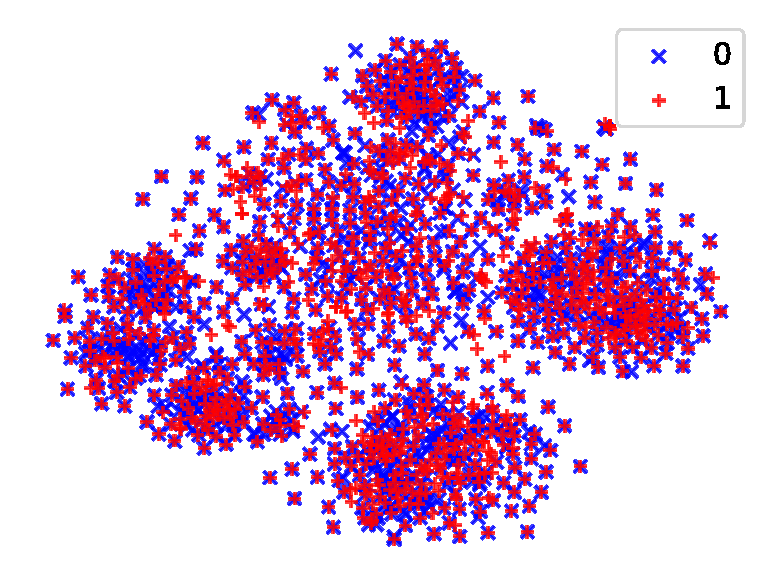
\includegraphics[width=3.5cm]{./images/ca_pre_c.pdf}
	\end{minipage}
	\begin{minipage}{0.45\linewidth}
		\centering
		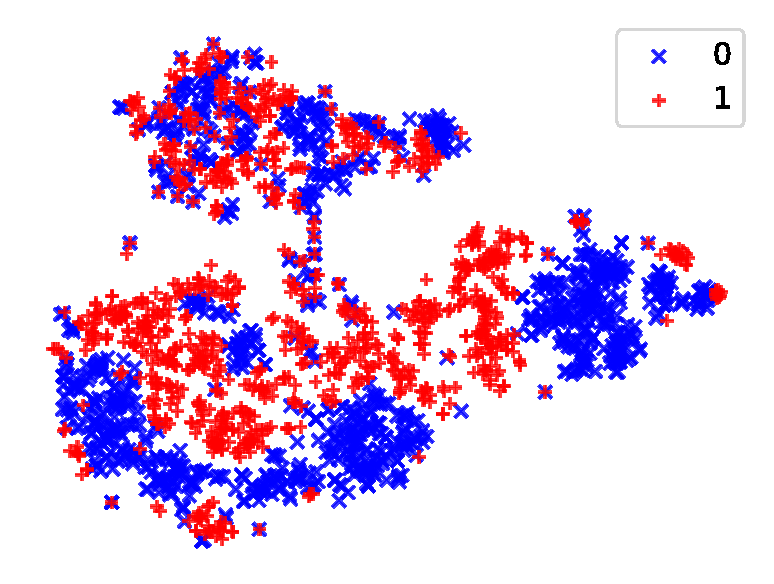
\includegraphics[width=3.5cm]{./images/ca_pre_s.pdf}
	\end{minipage}
	\underline{\small ST$^2$-CrossAlign}\\
	\begin{minipage}{0.45\linewidth}
		\centering
		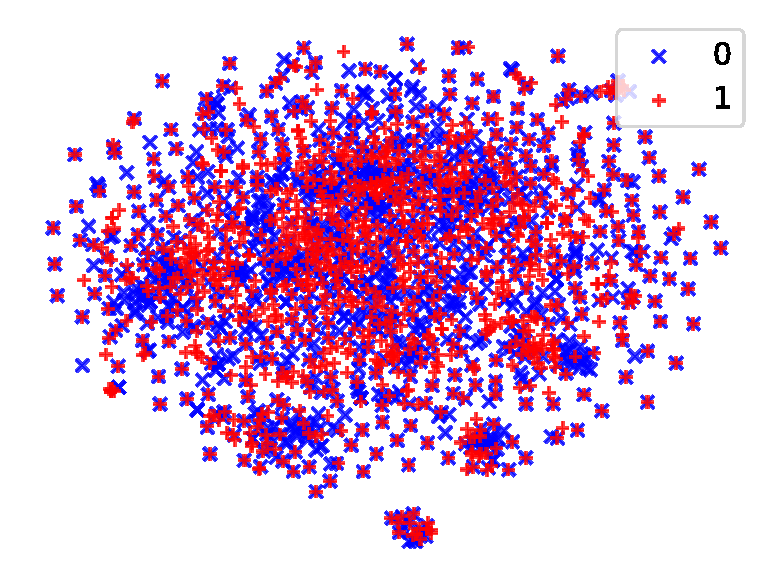
\includegraphics[width=3.5cm]{./images/ca_maml_c.pdf}
	\end{minipage}
	\begin{minipage}{0.45\linewidth}
		\centering
		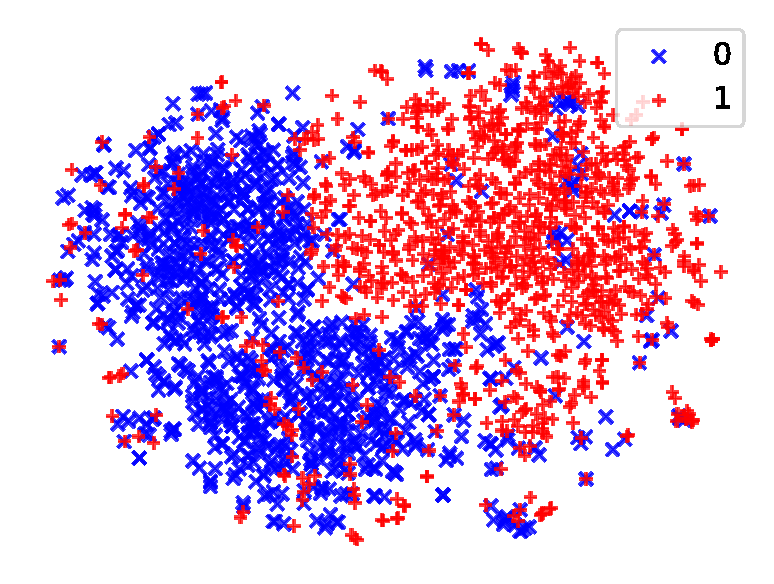
\includegraphics[width=3.5cm]{./images/ca_maml_s.pdf}
	\end{minipage}
	\underline{\small Pretrained VAE}\\
	\begin{minipage}{0.45\linewidth}
		\centering
		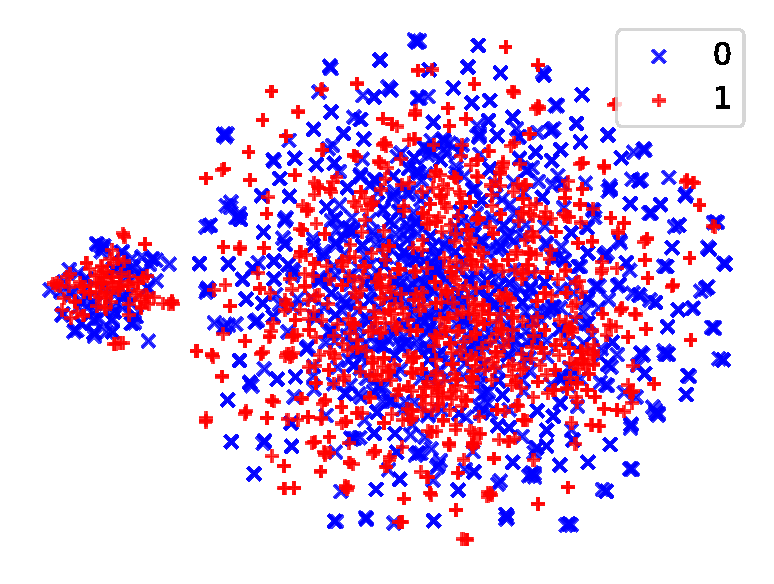
\includegraphics[width=3.5cm]{./images/vae_pre_c.pdf}
	\end{minipage}
	\begin{minipage}{0.45\linewidth}
		\centering
		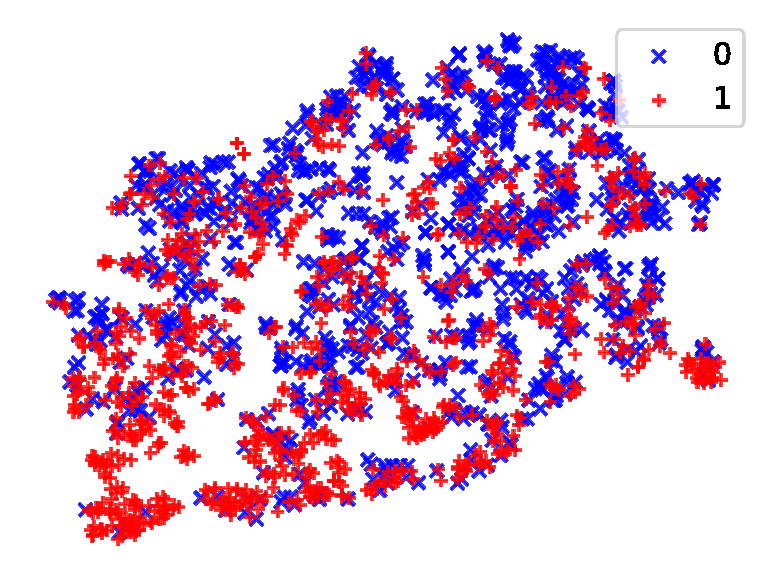
\includegraphics[width=3.5cm]{./images/vae_pre_s.pdf}
	\end{minipage}
	\underline{\small ST$^2$-VAE}\\
	\begin{minipage}{0.45\linewidth}
		\centering
		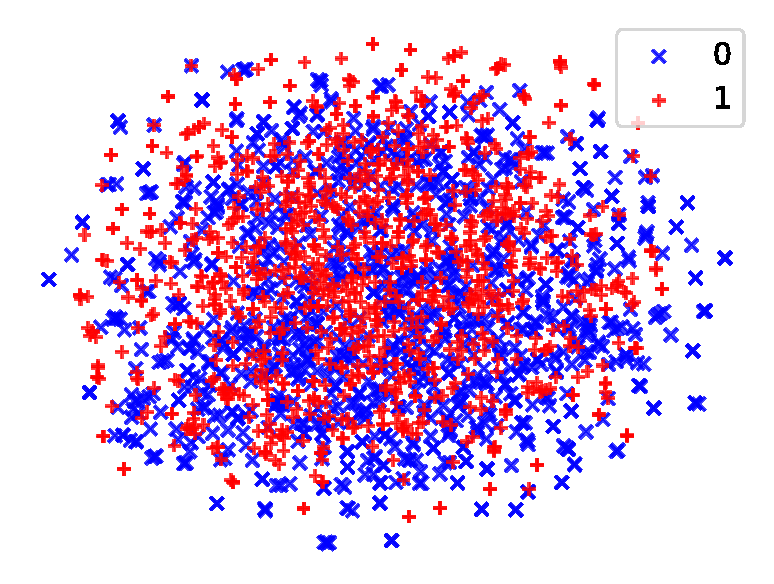
\includegraphics[width=3.5cm]{./images/vae_maml_c.pdf}
	\end{minipage}
	\begin{minipage}{0.45\linewidth}
		\centering
		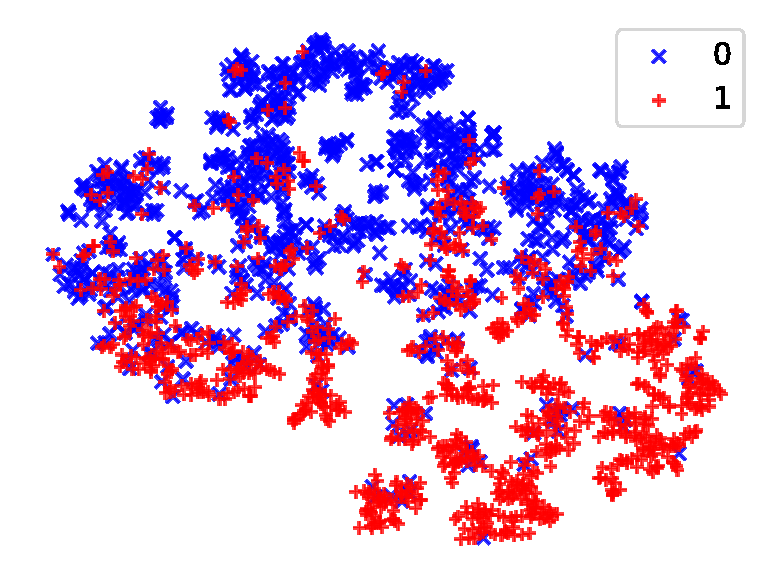
\includegraphics[width=3.5cm]{./images/vae_maml_s.pdf}
	\end{minipage}
	\caption{t-SNE plots for content(left) and style(right) embedding}\label{fig:tsne}
\end{figure}
By adding a pretraining phase, the models get a chance to see all the data and learn to generate fluent sentences via reconstruction. Therefore, it is not surprising that the content preservation measure (BLEU) and sentence naturalness measure (PPL) gives significantly better results than before but at a cost of style transfer accuracy. In effect, the models tend to reconstruct the original sentence and do not transfer the style. In comparison, our ST$^2$ model learns to generate reasonable sentences and transfer styles jointly in the training phase. Therefore, it is still superior in terms of style transfer accuracy. This verifies that the success of ST$^2$ is not merely resulted from a larger training dataset. The way that the model updates its knowledge is parallel, rather than sequential, which contributes to better language models and more effective style transfer.

Furthermore, we notice that the pretraining phase in our ST$^2$ model is not crucial, suggesting that it is the meta-learning framework that significantly contributes to the model's improvements in generating fluent sentences and effectively transferring styles.

\subsection{Disentanglement of Style}
\label{sec:disentangle}

Following the experiments adapted by \citet{john2018disentangled}, we use t-SNE plots as shown in Figure \ref{fig:tsne} to analyze the effectiveness of disentanglement of style embedding and content embedding in the latent space~\citep{maaten2008visualizing}. In particular, we compare the pretrained base models (CrossAlign and VAE) and our ST$^2$ models.




These two models, together with our ST$^2$ models attempt to disentangle style and content in latent space, and thus is well suited for this experiment, while it is unreasonable to treat hidden state vectors in other baseline models as content/style embedding. Therefore, they are excluded from this experiment.

As we can see from the figures, the content space learned by all models are relatively clustered, while the style spaces are more separated in our ST$^2$ models than the pretrained base models. This verifies that the improvements of meta-learning framework is not limited to a better language model, but also in terms of the disentanglement of styles.


